\section{Distributed Shared Memory}

Applications written for \Grappa utilize two forms of memory: local and
global. Local memory is local to a single core within a node in the system.
Accesses occur through conventional pointers. Applications use local accesses for a
number of things in \Grappa: the stack associated with a task, accesses to
localized global memory in caches (see below), and accesses to debugging
infrastructure local to each system node. Local pointers cannot access
memory on other cores, and are valid only on their home core.

Large data that is expected to be shared and accessed with low locality is
stored in \Grappa's global memory. All global data must be accessed through
calls into \Grappa's API, shown in Figure~\ref{fig:accessing-memory}.

\TODO{worth mentioning localized access for data-parallel stuff, along
    with reasoning about local vs remote accesses as in the PGAS world}

\paragraph{Global memory addressing} \Grappa provides two methods for storing
data in the global memory. The first is a distributed heap striped across all
the machines in the system in a block-cyclic fashion. The
\texttt{global\_malloc} and \texttt{global\_free} calls are used to allocate
and deallocate memory in the global heap. Addresses to memory in the global
heap use \emph{linear addresses}. Choosing the block size involves trading off
sequential bandwidth against aggregate random access bandwidth. Smaller block
sizes help spread data across all the memory controllers in the cluster, but
larger block sizes allow the locality-optimized memory controllers to provide
increased sequential bandwidth. The block size, which is configurable, is
typically set to 64 bytes, or the size of a single hardware cache line, in
order to exploit spatial locality when available.

\Grappa also allows any local data on a core's stacks or heap to be exported
to the global address space to be made accessible to other cores across the
system. Addresses to global memory allocated in this way use \emph{2D global
addresses}. This uses a traditional PGAS (partitioned global address
space~\cite{upc:2005}) addressing model, where each address is a tuple of a
rank in the job (or global process ID) and an address in that process. The
lower 48 bits of the address hold a virtual address in the process. The top
bit is set to indicate that the reference is a 2D address (as opposed to
linear address). This leaves 15~bits for network endpoint ID, which limits our
scalability to $2^{15}$ cores. Any node-local data can be made accessible
to other cores in the system by wrapping the address and node ID into a 2D
global address. This address can then be accessed with a delegate operation
and even be buffered by other cores. The address is converted at the destination
into a canonical x86 address by replacing the upper bits with the
sign-extended upper bit of the virtual address. 2D addresses may refer to
memory allocated from a single processes' heap or from a task's stack.
Figure~\ref{fig:memory-structure} shows how 2D and linear addresses can refer
to other cores' memory.


\begin{figure}[htbp]
  \begin{center}
    \begin{minipage}{0.95\columnwidth}
	\small
  \begin{description}
    \item[Allocation in the global heap:] \hfill \\
      	\lstinline[style=grappa]{GlobalAddress<T> global_malloc<T>( size )} \hfill \\
      	\lstinline[style=grappa]{global_free( GlobalAddress<T> )}  \hfill
    \item[Delegate operations:] \hfill \\
      	\lstinline|T    delegate_read( GlobalAddress<T>)|  \hfill \\
      	\lstinline|Promise<T> delegate_read_async( GlobalAddress<T> )|  \hfill \\
      	\lstinline|void delegate_write( GlobalAddress<T>, T value)| \hfill \\
      	\lstinline|void delegate_write_async( GlobalAddress<T>, T value)| \hfill \\
      	\lstinline|bool delegate_cas( GlobalAddress<T>, T cmp, T set)| \hfill \\
      	\lstinline|T    delegate_fetch_inc( GlobalAddress<T>, T inc)| \hfill \\
      	\lstinline|void delegate_inc_async( GlobalAddress<T>, T inc)|  \hfill\\ 
%        \lstinline|void buffer_acquire( GlobalAddress<T>, local_buf, {RO,RW,WO})| \hfill \\
%        \lstinline|void buffer_release( GlobalAddress<T>, local_buf )| \hfill
    % Perform buffer operations to acquire/release global data.
    % Acquire copies all data to local node and returns a pointer.
    % For write acquire, release copies data back to global memory.
	\end{description}
      \caption{\label{fig:accessing-memory} \Grappa API for memory accesses.}     \end{minipage}
  \end{center}
\end{figure}

\begin{figure}[t]
\begin{center}
  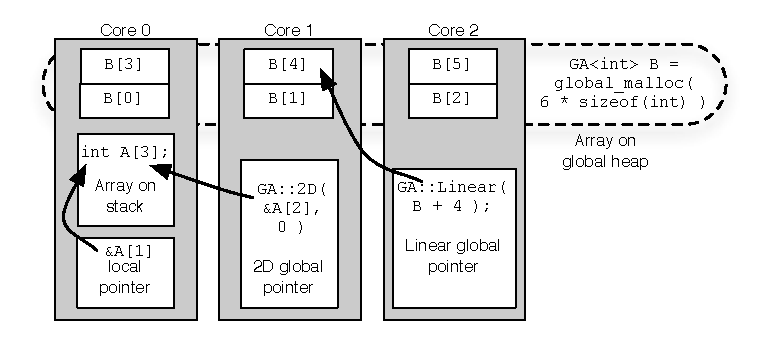
\includegraphics[width=0.95\columnwidth]{figs/memory-structure}
\begin{minipage}{0.95\columnwidth}
  \caption{\label{fig:memory-structure} Global memory referencing in \Grappa}
\end{minipage}
\vspace{-3ex}
\end{center}
\end{figure}

\paragraph{Global memory access} 
Access to \Grappa's distributed shared memory is provided through  {\em
delegate\/} operations, which are short memory accesses performed at the memory
location's home node. When the data access pattern has
low-locality, it is more efficient to modify the data on its home core rather
than bringing a copy to the requesting core and returning it after
modification. Delegate operations~\cite{Nelson:hotpar11, delegated:oopsla11}
provide this capability. Applications can dispatch computation to be performed
on individual machine-word sized chunks of global memory to the memory system
itself. Delegates can execute arbitrary non-blocking code, so we use them to perform simple
\emph{read\/}/\emph{write\/} operations to global memory, as well as more complex \emph{read-modify-write\/} operations (e.g., \emph{fetch-and-add\/}). 

Delegate operations are \emph{always\/} executed at the home core of their
address. The remote operation may not perform any operations that could cause
a context switch; this ensures any modifications are atomic. We limit delegate
operations to operate on objects in the 2D address space or objects that fit
in a single block of the linear address space so they can be satisfied with a
single network request. Given these restrictions, we can ensure that delegate
operations for the same address from multiple requesters are always serialized
through a single core in the system, providing atomic semantics without using
actual atomic operations (and thus avoiding their typical high cost).

Delegate operations can be either {\em blocking\/} or {\em non-blocking}.
With blocking operations, the task issuing the delegate call blocks until
the delegate operation completes, which is necessary, for example, to ensure
that synchronization has finished before continuing. Synchronization in \Grappa
is implemented using blocking delegate operations. On the other hand, remote data
accesses often can overlap. In order to avoid
unnecessary waiting, we support non-blocking delegate operations. For reads,
we support a ``futures''-like mechanism. Tasks may issue delegate reads in
parallel and block on the ``promises'' returned by non-blocking delegate
invocations. Delegate write operations may also be performed as
non-blocking,
and since they do not return data, a mechanism to detect completion is needed.
\Grappa provides a \texttt{GlobalCompletionEvent} synchronization object, which non-blocking operations (including tasks) can be enrolled with and which other tasks can block on to be notified and woken when all enrolled operations in the collection are complete.
\TODO{augment this with our bulk futures ie global completions}

When programmers want to operate on data structures spread across
multiple nodes, accesses must be expressed as multiple delegate
operations along with with appropriate synchronization
operations. \Grappa's API also includes calls for gathering and scattering
contiguous blocks in the global heap, but the user is responsible for
ensuring correct synchronization.

\paragraph{Memory consistency model discussion} As mentioned earlier, all
synchronization operations are done via delegate operations. Since they all
execute on their home core in some serial order, they are guaranteed to be globally linearizable~\cite{herlihy1990linearizability}, with their
updates visible to all cores across the system in the same order. In addition, only one synchronous delegate will be in flight at a time from a particular task. Therefore, synchronization operations from a particular task are not subject to reordering. 
% \TODO{I think we can support multiple delegates in parallel from a task as
% long as we block on them before counting on them being complete. see my
% description above about the \emph{future/promise} delegates we have now. Not
% sure if there's a strong example of when this is useful for synchronization
% (though it's definitely useful for reads/writes), acquiring multiple locks
% doesn't work because we have to acquire locks in order to prevent deadlock.}
Consequently, all synchronization operations execute in program order and are
made visible in the same order to all cores in the system. These properties
are sufficient to guarantee a memory model that offers sequential consistency
for data-race-free programs~\cite{AdveHill1990} (all accesses to shared data
are separated by synchronization). This is the memory model that underpins
C/C++~\cite{N2480,N2800}.

Note, however, that if the application code uses explicit buffers or
asynchronous delegates to access shared data, all updates must be published back to
the home core before the synchronization operation that protects the data is
performed. This is done using release operations on cached regions and using
the \texttt{GlobalCompletionEvent} object to determine that asynchronous
delegates have completed.



\TODO{admit the lack of a synchronization feature for lightweight
    transactions across two or more domains. Talk about using the same
    philosophy of moving data along with the sync (same as a real
    cache) and utilizing latency tolerance. Then say further is out of
    scope for this paper.}

